%!TEX root = ../main.tex

\section{The system of neutral \texorpdfstring{$\Bd$}{B0} mesons}
\label{sec:cpviolation:neutralBmesons}

In the system of neutral \Bd mesons four decay amplitudes occur. The decay
amplitude \Af stands for the decay of a \Bd meson into a final state $f$, while
\Abarf is the decay amplitude of an \Bdb meson into the same final state.
Similarly, the decay amplitudes into the \CP-conjugated final state $\bar{f}$
can be defined. By convention \Bd mesons consist of \bquarkbar and \dquark
quarks, while \Bdb mesons contain \bquark and \dquarkbar quarks. These two
mesons can mix, \ie they can oscillate between the two flavour states. As
flavour-changing neutral currents (FCNC) are forbidden in the SM, the
\Bd--\Bdb oscillation is in lowest order Standard Model described by quantum
loops involving charged currents as shown in the Feynman diagrams in
\cref{fig:cpviolation:neutralBmesons:boxdiagram}.
\begin{figure}[htb]
\centering
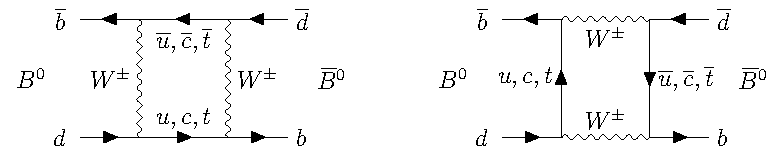
\includegraphics[width=\textwidth]{03-CPViolation/tikz/pdf/Boxdiagrams.pdf}
\caption{Box diagrams of \Bd--\Bdb oscillation.}
\label{fig:cpviolation:neutralBmesons:boxdiagram}
\end{figure}
The corresponding decay amplitude is given by
\begin{align}
	\mathcal{A}(\Bdb\!\to\Bd) \propto \frac{g_2^4}{16\,\pi^2}(\Vtb\Vtds)^2 \frac{\bra{\Bd}(\dquarkbar_L\gamma_\mu\bquark_L)(\dquarkbar_L\gamma^\mu\bquark_L)\ket{\Bdb}}{M_W^2}S(x_t)\,,
\label{eq:cpviolation:mixingamplitude}
\end{align}
\todo{probably typo in book}
with the \W boson mass $M_W$, the squared fraction of the top quark mass $x_t
= m_t^2/M_W^2$ and the Inami-Lim function~\cite{Inami:1980fz}
\begin{align}
	S(x_t) = x_t \left(\frac 14 + \frac 94 \frac{1}{1 - x_t} - \frac 32 \frac{1}{(1 - x_t)^2}\right) + \frac 32 \left(\frac{x_t}{x_t - 1}\right)^3 \log x_t\,.
\label{eq:cpviolation:inamilim}
\end{align}
Here, it is accounted for the suppression of contributions with up and charm
quarks in the loop due to $m_{\uquark,\cquark}^2 \ll m_{\tquark}^2$. Formulae
(\ref{eq:cpviolation:mixingamplitude}) and (\ref{eq:cpviolation:inamilim}) are
taken from Ref.~\cite{Brock:2011zz}.

To derive the time evolution of initially produced \Bd and \Bdb mesons the
Schrödinger equation~\cite{Schroedinger} needs to be solved. Assuming the
Wigner-Weisskopf approximation~\cite{Weisskopf:1930au,*Weisskopf:1930ps}, \ie
(excited) states do not know about their past, which is valid since the time
scale of weak decays is significantly larger than the time scale of the
production via the strong force, the effective Schrödinger equation for the
wave function representing the system of \Bd and \Bdb mesons can be written as
\begin{align}
	i \frac{\mathrm{d}}{\mathrm{dt}}
\begin{pmatrix}
	\ket{\Bd(t)}	\\	\ket{\Bzb(t)}	
\end{pmatrix}
	= \matr{H}
\begin{pmatrix}
	\ket{\Bd(t)}	\\	\ket{\Bzb(t)}	
\end{pmatrix}
	= \left(\matr{M} - i \frac{\matr{\Gamma}}{2}\right)
\begin{pmatrix}
	\ket{\Bd(t)}	\\	\ket{\Bzb(t)}
\end{pmatrix}
\,.
\end{align}
The Hamiltonian \matr{H} is given by a non-Hermitian matrix, otherwise only
oscillations but no decays would occur. It consists of Hermitian $2\times2$
mass \matr{M} and decay matrices \matr{\Gamma}, which have contributions from
virtual intermediate states respectively from physical final states accessible
by both \Bd and \Bdb. Due to the \CPT theorem the diagonal elements of
\matr{M} and \matr{\Gamma} are equal, \ie $M_{11} = M_{22}$ and $\Gamma_{11} =
\Gamma_{22}$. The non-zero off-diagonal elements, else there would be no
mixing, cause that the flavour eigenstates \Bd and \Bdb are not mass
eigenstates. Instead, the light ($L$) and heavy ($H$) mass eigenstates are
given by the linear combinations
\begin{align}
\begin{split}
	\ket{B_L} = p \ket{\Bd} + q \ket{\Bdb} \,,\\
	\ket{B_H} = p \ket{\Bd} - q \ket{\Bdb} \,,
\end{split}
\label{eq:cpviolation:neutralBmesons:superposition}
\end{align}
with the complex coefficients $p$ and $q$, which fulfil the normalisation
condition $|p|^2 + |q|^2 = 1$ and whose ratio can be expressed with the matrix
elements as
\begin{align}
	\frac qp = \sqrt{\frac{2M_{12}^\ast - i\Gamma_{12}^\ast}{2M_{12} - i\Gamma_{12}}}\,.
\label{eq:cpviolation:qp}
\end{align}
Explicit calculations of $\Gamma_{12}$, as performed in
Ref.~\cite{Buras:1984pq}, show that to a very good approximation
\cref{eq:cpviolation:qp} can be simplified to
\begin{align}
	\frac qp \approx \sqrt{\frac{M_{12}^\ast}{M_{12}}} = \frac{\Vtbs\Vtd}{\Vtb\Vtds}\,.
\label{eq:cpviolation:qp_simplified}
\end{align}

The well-defined masses and decay widths
$m_{L,H}$ and $\Gamma_{L,H}$ of $B_L$ and $B_H$ lead to the eigenvalues
\begin{align}
\begin{split}
	\mu_L &= m_L - \sfrac{i}{2}\Gamma_L \,,\\
	\mu_H &= m_H - \sfrac{i}{2}\Gamma_H \,,
\end{split}
\end{align}
which can be used to shortly express the time-evolution of the mass eigenstates
\begin{align}
	\ket{B_{L,H}(t)} = e^{-i\mu_{L,H}t} \ket{B_{L,H}}\,.
\end{align}
Using \cref{eq:cpviolation:neutralBmesons:superposition} the time evolution of
$B$ mesons purely produced as \Bd or \Bdb can be derived
\begin{align}
\begin{split}
	\ket{\Bd(t)} = g_+(t)\ket{\Bd}  + \frac qp g_-(t)\ket{\Bdb}\,,\\
	\ket{\Bd(t)} = g_+(t)\ket{\Bdb} + \frac pq g_-(t)\ket{\Bd} \,,
\end{split}
\label{eq:cpviolation:Btimeevolution}
\end{align}
with the time-dependent coefficients
\begin{align}
\begin{split}
	g_+(t) = e^{-i\frac{\mu_L + \mu_H}{2}t}\left[+\cosh\frac{\DGd\,t}{4} \cos\frac{\dmd\,t}{2} - i \sinh\frac{\DGd\,t}{4} \sin\frac{\dmd\,t}{2}\right]\,,\\
	g_-(t) = e^{-i\frac{\mu_L + \mu_H}{2}t}\left[-\sinh\frac{\DGd\,t}{4} \cos\frac{\dmd\,t}{2} + i \cosh\frac{\DGd\,t}{4} \sin\frac{\dmd\,t}{2}\right]\,.
\end{split}
\label{eq:cpviolation:gplusgminus}
\end{align}
The mass difference $\dmd = m_H - m_L$ drives the oscillation and can be
interpreted as mixing frequency, while $\DGd = \Gamma_H - \Gamma_L$ is
negligible in the \Bd meson sector~\cite{HFAG}.

The differential decay rates, \ie the squared decay amplitudes, can be
expressed by combining the terms in
\cref{eq:cpviolation:Btimeevolution,eq:cpviolation:gplusgminus} as
\begin{align}
\begin{split}
	\Gamma(\Bd(t)\to f) &= |\Af|^2 \Big\{|g_+(t)|^2 + |\lambda_f|^2|g_-(t)|^2 + 2\,Re[\lambda_f g_+^\ast(t)g_-(t)]\Big\}\,,\\
	\Gamma(\Bzb(t)\to f) &= |\Af|^2 \left|\frac pq \right|^2 \Big\{|g_-(t)|^2 + |\lambda_f|^2|g_+(t)|^2 + 2\,Re[\lambda_f g_+(t)g_-^{\ast}(t)]\Big\}\,,
\end{split}
\label{eq:cpviolation:complexdecayrates}
\end{align}
using
\begin{align}
	\lambda_f = \frac qp \frac{\Abarf}{\Af}\,.
\label{eq:cpviolation:lambda}
\end{align}
